\def\difficulty{3}
\sujet{Morphological Geodesic Filtering}\index{Mathematical Morphology!Geodesic Filtering}
\begin{note}This tutorial aims to test different morphological filters and particularly the geodesic ones (using reconstruction) for gray-level images.
\end{note}


\noindent The different processes will be applied on the following images:
{
	\makeatletter
	\renewcommand\fs@ruled{\def\@fs@cfont{\bfseries}\let\@fs@capt\floatc@ruled
		\def\@fs@pre{\hrule height.8pt depth0pt \kern2pt}%
		\def\@fs@post{\kern2pt\hrule\relax}%
		\def\@fs@mid{\vskip2pt}%
		\let\@fs@iftopcapt\iftrue}
	\makeatother
\begin{figure}[htbp]
\centering
\subfloat[Lena]{
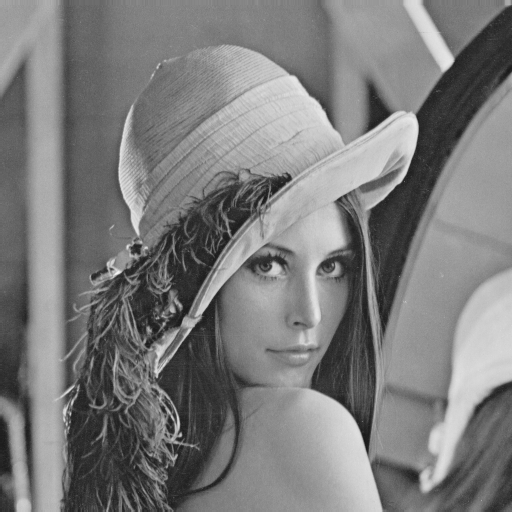
\includegraphics[width=4.25cm]{lena.png}}\hspace*{1cm}
\subfloat[2-D section of a cement paste (X-ray tomography)]{
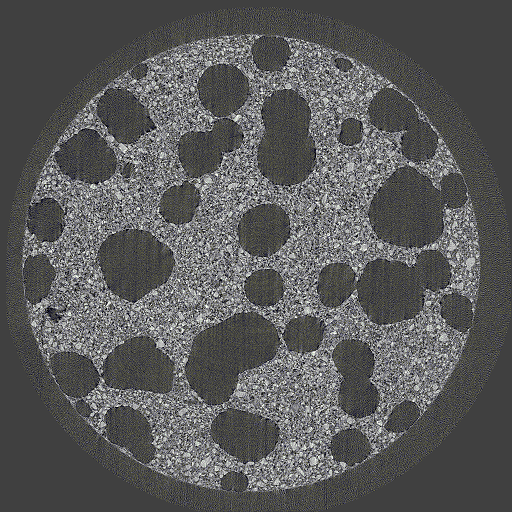
\includegraphics[width=4.25cm]{ciment.png}}
%\caption{Illustration of 2-D Boolean models observed in a squared window $W$.}
%\label{fig:images}
\end{figure}
}


\section{Morphological centre}
The morphological centre is an auto-dual filter using a family of operators $\{\psi_i\}_i$:
\begin{eqnarray}
C(f)=(f \vee (\wedge\{\psi_i(f)\})) \wedge (\vee\{\psi_i(f)\})
\end{eqnarray}
\begin{qbox}
\begin{itemize}
	\item Implement this transformation with the family $\{\gamma\phi\gamma, \phi\gamma\phi\}$ where $\gamma$ denotes the morphological opening and $\phi$ the morphological closing.
	\item Test this operator by varying the size of the structuring element.
	\item Add a 'salt and pepper' noise to the 'Lena' image and compare the morphological center with the median filtering.
	\item Try to reduce the noisy image 'cement paste'.
\end{itemize}
\end{qbox}

\section{Alternate sequential filters (ASF)}\index{Mathematical Morphology!Alternate Sequential Filters}
ASF can be defined from a family of openings and closings:
\begin{eqnarray}
N_i(f)&=&\gamma_i\phi_i\circ\gamma_{i-1}\phi_{i-1}\dots\gamma_2\phi_2\circ\gamma_1\phi_1(f)\\
M_i(f)&=&\phi_i\gamma_i\circ\phi_{i-1}\gamma_{i-1}\dots\phi_2\gamma_2\circ\phi_1\gamma_1(f)
\end{eqnarray}
where $\gamma_k$ (resp. $\phi_k$) denotes the opening (resp. closing) with a structuring element of size $k$.
\begin{qbox}
\begin{itemize}
	\item Implement these two operators.
	\item Test these transformations on the noisy image by varying the parameter $i$ of the filter.
\end{itemize}
\end{qbox}

\section{Reconstruction filters}\index{Mathematical Morphology!Reconstruction}
The geodesic dilation of size $1$ and $n$ are respectively defined as:
\begin{eqnarray}
\delta_f(g)&=&\wedge(\delta_{B_1}(g),f)\\
\delta_f^{n}(g)&=&\delta_f(\delta_f\dots(\delta_f(g)))
\end{eqnarray}
where $\delta_{B_1}$ denotes the morphological dilation with a disk of radius $1$ as structuring element.
The opening ($\gamma_k^{rec}(f)$) and closing ($\phi_k^{rec}(f)$) by reconstruction are then defined as:
\begin{eqnarray}
\gamma_k^{rec}(f)&=&\vee\{\delta_f^{n}(\epsilon_{B_k}(f)),n>0\}\\
\phi_k^{rec}(f)&=&M-\gamma_k^{rec}(M-f)
\end{eqnarray}
where $\epsilon_{B_k}$ denotes the morphological erosion with a disk $B$ of radius $k$ as structuring element.
\begin{qbox}
\begin{itemize}
	\item Implement these two operators $\gamma_k^{rec}(f)$ and $\phi_k^{rec}(f)$.
	\item Test these transformations by varying the parameter $k$ of the filter.
	\item Implement and test (on the noisy image) the filters of morphological center and ASF using the geodesic operators. Compare with the classical ones.
\end{itemize}
\end{qbox}
